\section{Benchmark NIST-1 "Analytic Solution"}
\label{sec:bench-1}

This is the first benchmark problem with a smooth solution
that is used for testing adaptive algorithms performance
where adaptivity isn't really needed.
The equation solved is the Poisson's equation.

\begin{equation} \label{poisson}
-\Delta u = f,
\end{equation}
in the domain $\Omega = (0, 1)^2$, equipped with Dirichlet
boundary condition given by the exact solution.
The exact solution $u(x, y) = 2^{4p}x^{p}(1-x)^{p}y^{p}(1-y)^{p}$
of this problem is shown in Fig. \ref{fig:sln-nist01}.
Here $p$ is a parameter, determining the polynomial degree of the exact solution.

\begin{figure}[!ht]
\centering
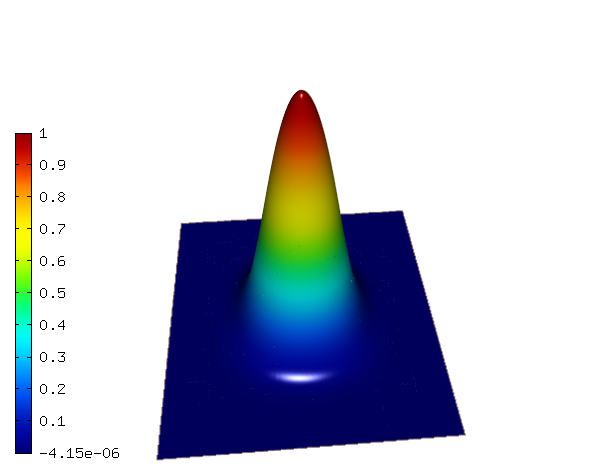
\includegraphics[height=5cm]{nist/nist-1/solution.png}
\caption{The solution to NIST-1 benchmark problem.}
\label{fig:sln-nist01}
\end{figure}
\noindent
The goal of the benchmark is to reach a relative error below
$10^{-2}$~\% in the $H^1$-norm with as few degrees of freedom (DOF)
as possible.
We begin with adaptive $hp$-FEM with possibly anisotropic refinements (adaptivity mode
HP\_ANISO\_H in {\sc Hermes}). The initial mesh is shown in Fig. \ref{fig:nist-1-hp-aniso} (left).
In a few adaptivity steps, the polynomial degree of this domain is increased
anisotropically.
The resulting mesh with 769 DOF is shown in Fig. \ref{fig:nist-1-hp-aniso} (right).

\begin{figure}[!ht]
\centering
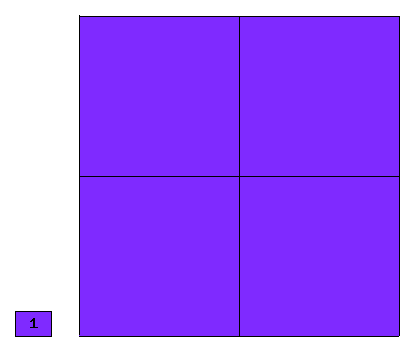
\includegraphics[height=5cm]{nist/nist-1/mesh_hp_aniso_init.png}\ \
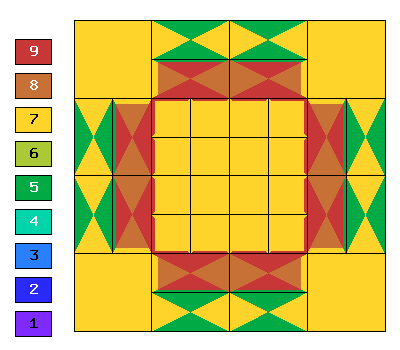
\includegraphics[height=5cm]{nist/nist-1/mesh_hp_aniso.png}
\vspace{-2mm}
\caption{Initial mesh (left) and final mesh (right) for $hp$-FEM with anisotropic refinements.}
\label{fig:nist-1-hp-aniso}
\end{figure}

The final relative error estimate in $H^1$-norm was 3.91108e-03 \%,
and it was identical to the exact error in all printed digits.
We also solved this benchmark with adaptive $h$-FEM
with linear (left) and quadratic (right)
elements, with anisotropic refinements enabled.
Final meshes for the $h$-FEM computations are shown
in Fig. \ref{fig:nist-1-h-aniso}.

\begin{figure}[!ht]
\centering
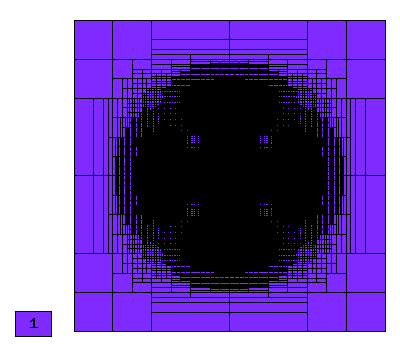
\includegraphics[height=5cm]{nist/nist-1/mesh_h1_aniso.png}\ \
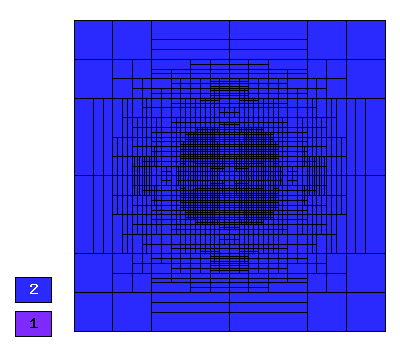
\includegraphics[height=5cm]{nist/nist-1/mesh_h2_aniso.png}
\vspace{-2mm}
\caption{Final mesh for $h$-FEM anisotropic refinements with linear and quadratic elements.}
\label{fig:nist-1-h-aniso}
\end{figure}

Figs. \ref{fig:nist-1-conv} compare all
three approaches to automatic adaptivity  from the point
of view of DOF and CPU convergence.

\begin{figure}[!ht]
\centering
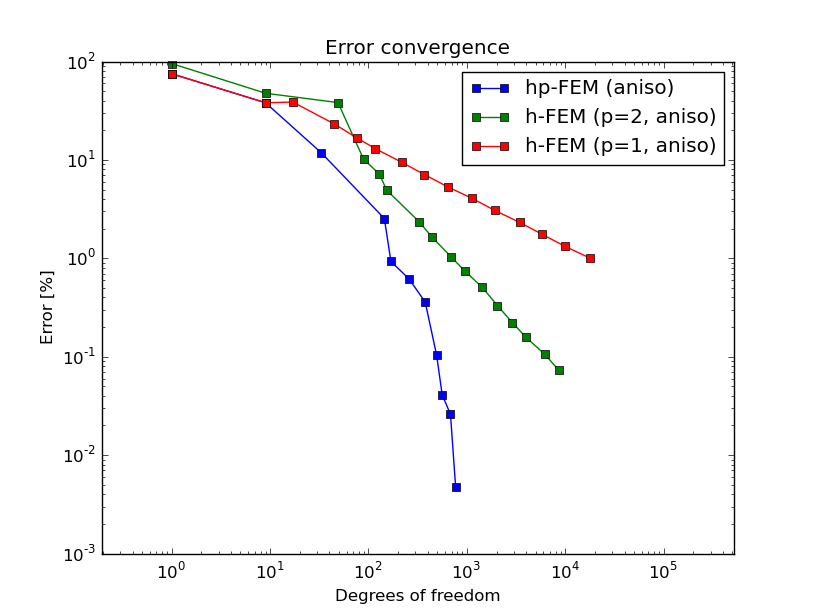
\includegraphics[height=5cm]{nist/nist-1/conv_dof_aniso.png}\ \
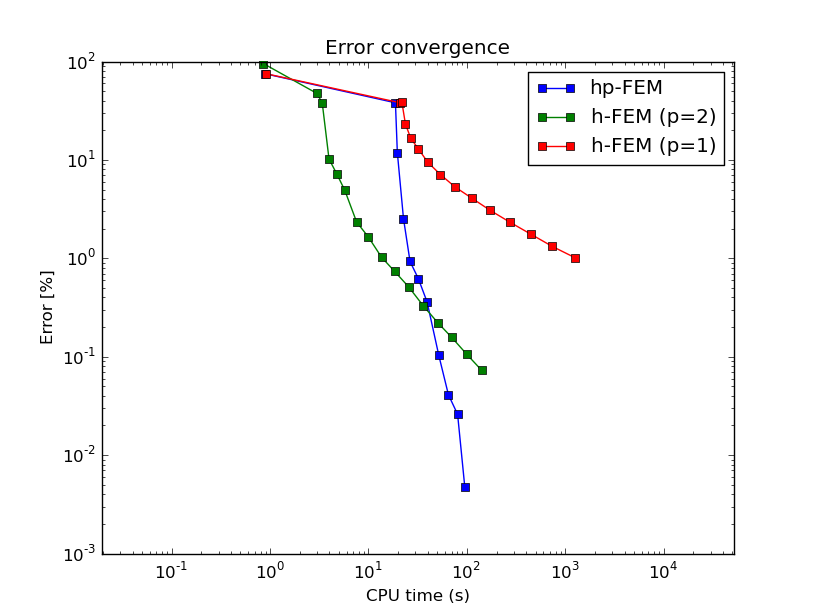
\includegraphics[height=5cm]{nist/nist-1/conv_cpu_aniso.png}
\vspace{-2mm}
\caption{DOF and CPU time convergence graphs.}
\label{fig:nist-1-conv}
\end{figure}
